% In this experiment, we will subject the RLC circuit to a sinusoidal input
% voltage and observe the response of the circuit. We will also measure the
% frequency response of the circuit.
% The RLC circuit has applications in electronics. It is used as a filter for
% tuning radio frequencies, for example.

% In order to obtain the total impedance of the series RLC circuit, we write:
% \begin{equation}
%     Z_S = R_S + j \omega L + \frac{1}{j \omega C}
% \end{equation}
% The admittance of the circuit, equivalently is:
% \begin{equation}
%     Y_P = G_P + j\omega C + \frac{1}{j \omega L}
% \end{equation}
% Where the absolute value of the impedance is given as:
% \begin{equation}
%     |Z_S| = \sqrt{R_S^2 + \left( \omega L - \frac{1}{\omega C} \right)^2}
% \end{equation}

% \begin{figure}[htbp]
%     \centering
%     \begin{subfigure}[h]{0.45\textwidth}
%         \centering
%         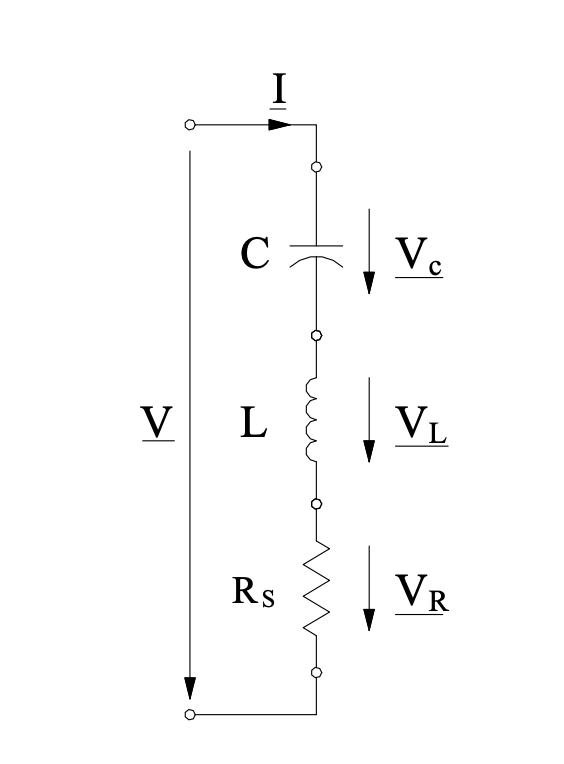
\includegraphics[width=0.8\textwidth]{images/series_RLC.png}
%         \caption{Series RLC Circuit}
%         \label{fig:figure1}
%     \end{subfigure}\hfill%
%     \begin{subfigure}[h]{0.45\textwidth}
%         \centering
%         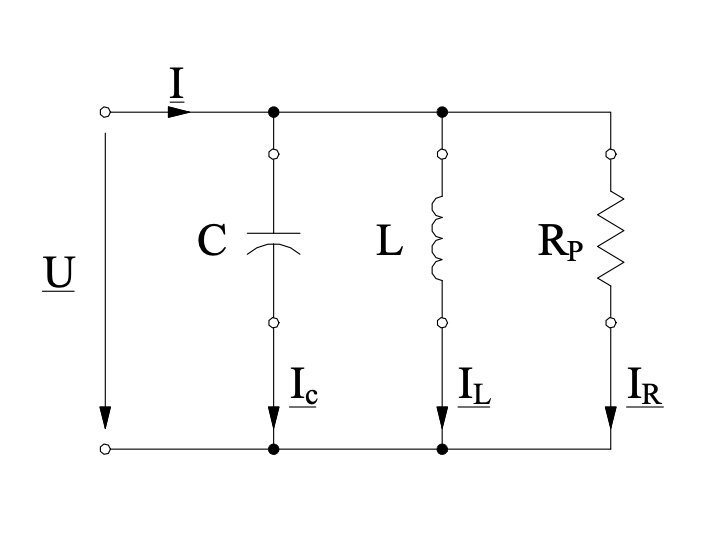
\includegraphics[width=0.8\textwidth]{images/parallel_RLC.png}
%         \caption{Parallel RLC Circuit}
%         \label{fig:figure2}
%     \end{subfigure}
%     \label{fig:main}
% \end{figure}

% The complex phase of the impedance is given by
% \begin{equation}
%     \varphi = \arctan \left(\frac{\omega L - 1/ \omega C}{R_s}\right)
% \end{equation}
% Where the general representation for an impedance is given by:
% \begin{equation}
%     Z(\omega) = R + jX(\omega)
% \end{equation}
% When we have resonance, we denote $\omega$ as $\omega_0$, and when $\omega = \omega_0$ the impedance is purely real:
% \begin{equation}
%     Im(Z(\omega_0)) = 0 \implies Z(\omega_0) = Re(Z(\omega_0)) = R
% \end{equation}

% {\bf On reactive power:} Reactive power consumed by the circuit varies mostly on whether the RLC circuit is in series or in parallel.

% In {\bf series}, the reactive power is minimized when the circuit is driven by a current source, and maximized when driven by a voltage source.

% In {\bf parallel}, the reactive power is minimized when the circuit is driven by a voltage source, and maximized when driven by a current source.

% \vspace{1cm}
% {\bf Bandwidth and quality factor:} The bandwidth is a measure of the frequency
% selectivity of a resonating circuit. The bandwidth $B$ of the resonators can directly
% be extracted either from the magnitude or the phase plot.
% In the magnitude plot, the bandwidth corresponds to the full width of the curve at half maximum,
% which means that the magnitude is dropped by a factor of 2. From the phase plot, the bandwidth $B$
% can be extracted by taking the difference of the phase between $\pi/4$ and $-\pi/4$
% Furthermore, the bandwidth can be determined by mathematical means.
% For example, in a series RLC circuit, the bandwidth is given by:
% \begin{equation}
%     B = \omega _2 - \omega _1 = \frac{R_s}{L}
% \end{equation}

% Where we obtain this result by knowing that
% \begin{equation}
%     \omega _1 = -\frac{R_s}{2L} + \sqrt{\left(\frac{R_s}{2L}\right)^2+\frac{1}{LC}}
% \end{equation}

% And we know that $\omega _2$ is the frequency at which the impedance is equal to $R_s$:
% \begin{equation}
%     \omega _2 = \frac{R_s}{2L} + \sqrt{\left(\frac{R_s}{2L}\right)^2+\frac{1}{LC}}
% \end{equation}

% And the quality factor is given by:
% \begin{equation}
%     Q = \frac{X_0}{R_s} = \frac{\omega _0}{B}
% \end{equation}

% Where $\omega _0$ is obtained by $\omega _0 = \frac{1}{\sqrt{LC}}$ and $X_0$ can be defined as:
% \begin{equation}
%     X_0 = \omega _0 L = \frac{1}{\omega _0 C}
% \end{equation}

% {\bf \large Prelab:}

\begin{figure}[htbp]
    \centering
    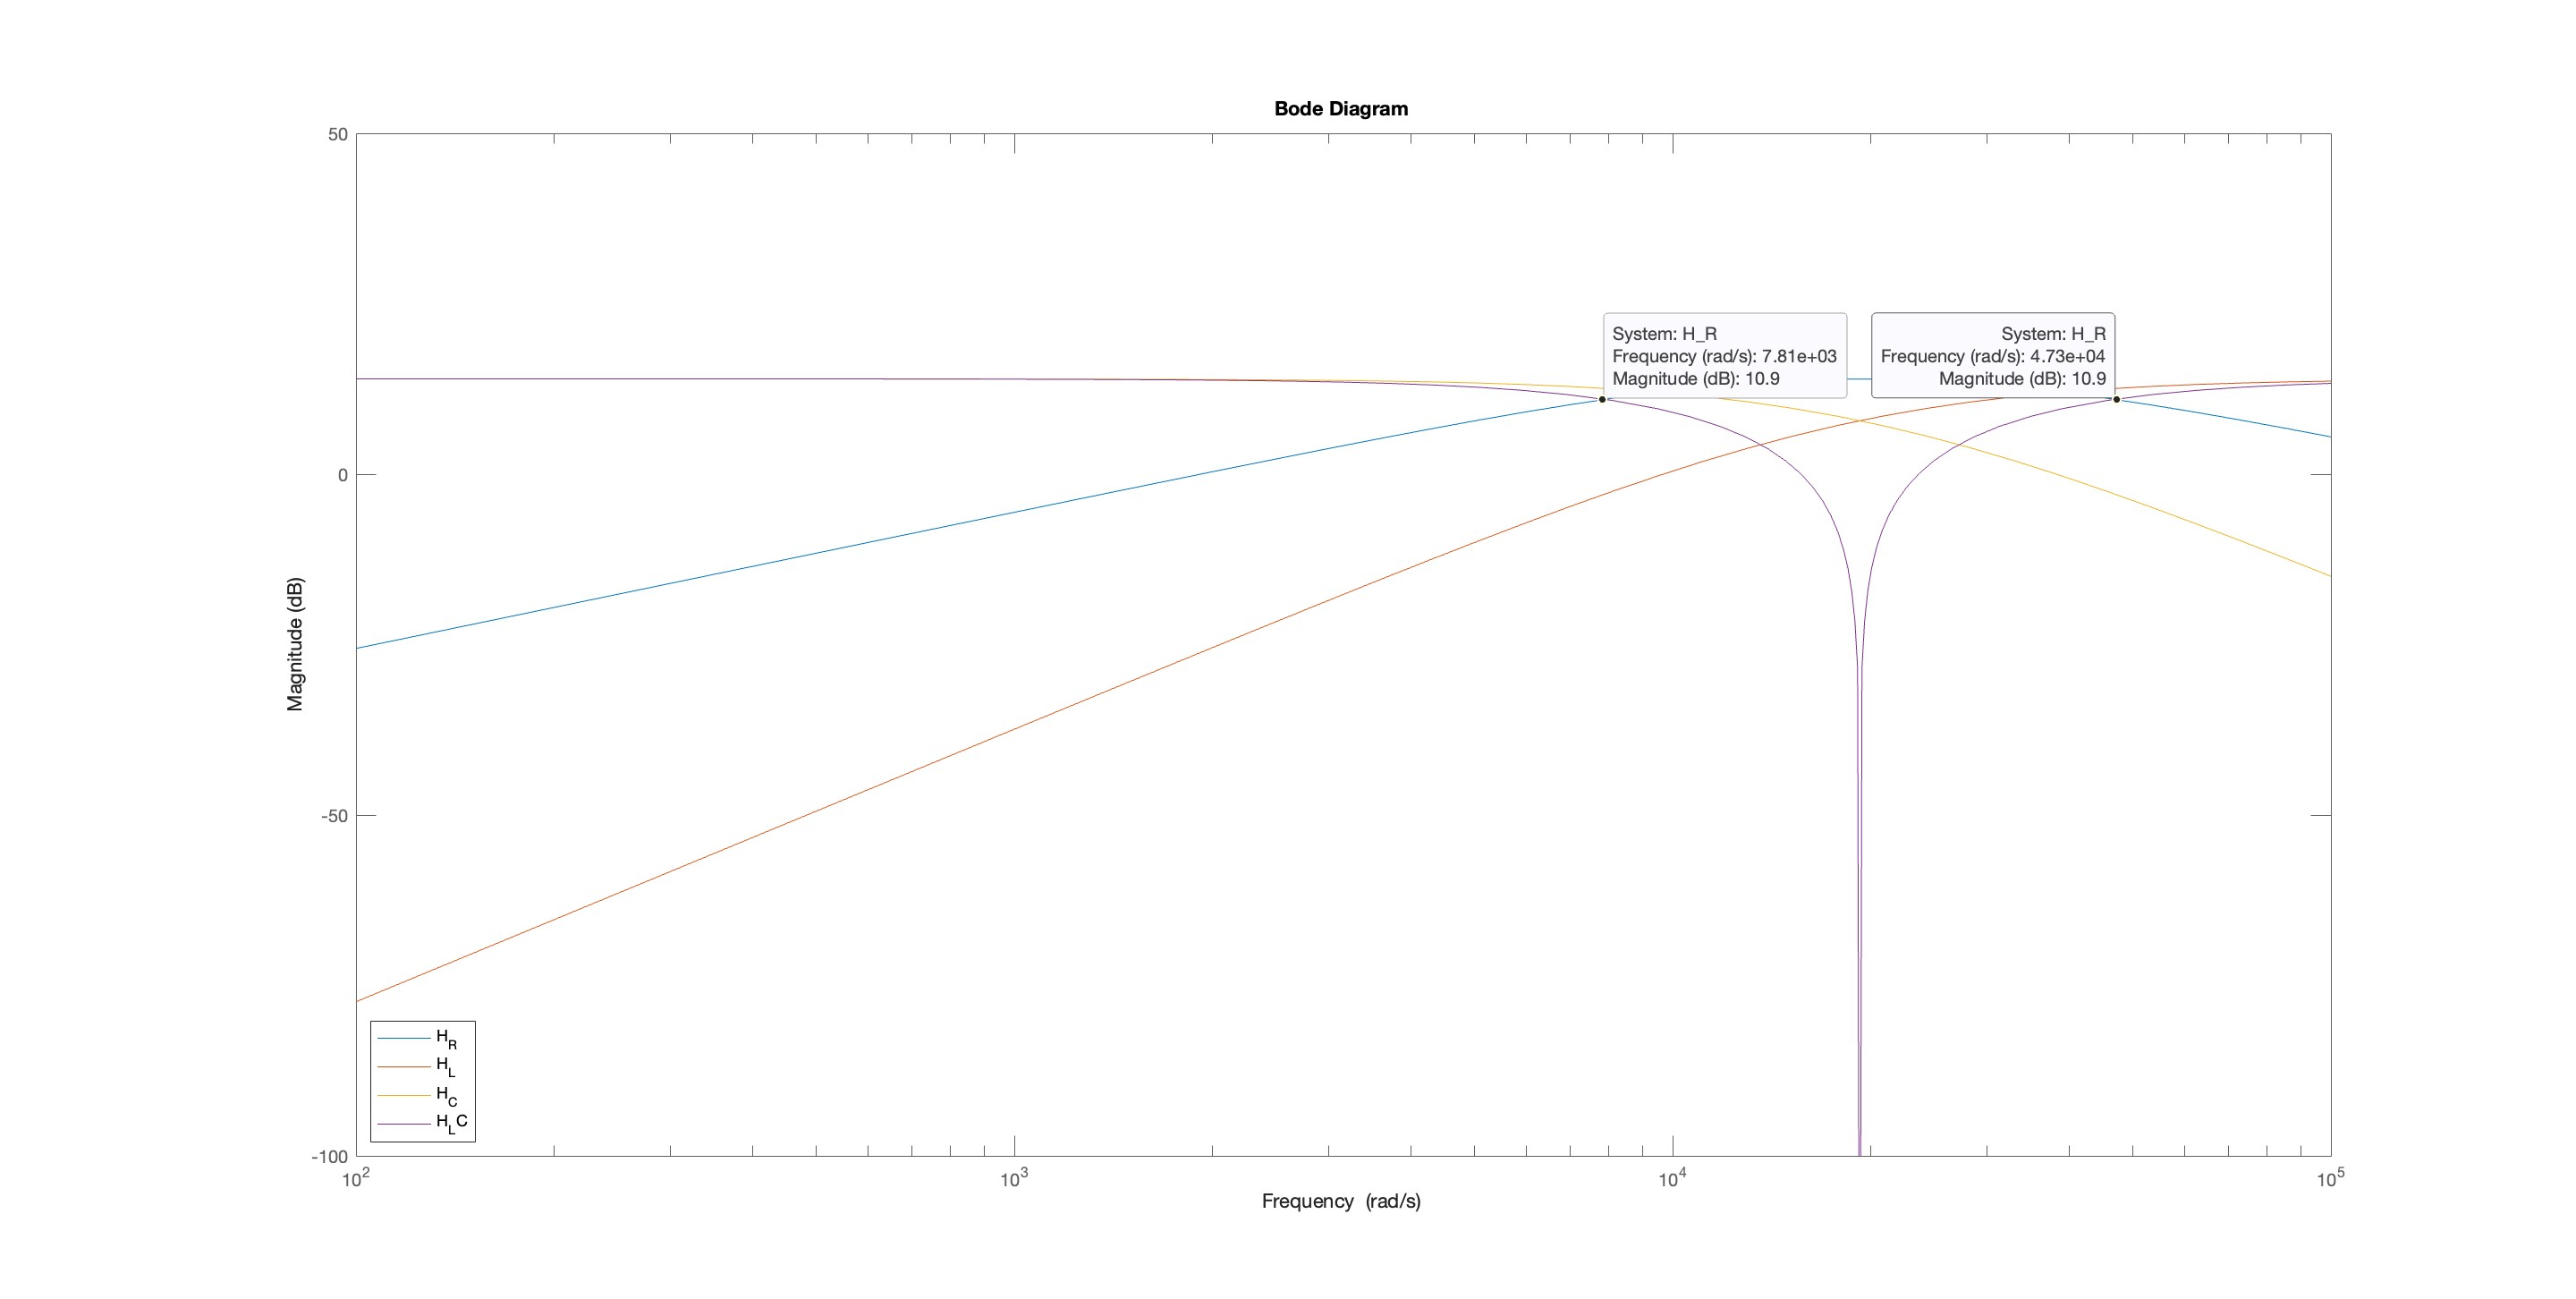
\includegraphics[width=\textwidth]{images/parallel_RLC_series_plot.jpg}
    \caption{RLC Series Voltages taken over different components}
    \label{fig:prelab}
\end{figure}

From the plot, we find that the corner frequencies are given as
\begin{equation}
    \omega _1 = 7.81E3 \text{ rad/s} \text{ and } \omega _2 = 4.73E4 \text{ rad/s}
\end{equation}


We also find that the bandwidth is, in the series RLC circuit:

\begin{center}
    {\bf Calculated}: $3.9E4$
    \\
    {\bf Plotted}: $3.94E4$
\end{center}

The quality factor is calculated to be(by knowing that $Q = \frac{X_0}{R} = \frac{\sqrt{\frac{L}{C}}}{R}$)

\begin{center}
    \(Q=0.49346\)
\end{center}

We find that the voltage taken over the resistor makes the circuit act as a {\bf bandpass} filter, the voltage taken over the
inductor makes the circuit act as a {\bf high-pass} filter,
the voltage taken over the capacitor makes the circuit act as a {\bf low-pass} filter, and the voltage taken over the inductor and the capacitor makes the circuit act as a {\bf band-stop} filter.
The bode magnitude of the RLC series circuit plot and the MATLAB code used to obtain the corner frequencies and create the plot is given below:
\begin{verbatim}
R = 390; % in ohm
C = 270E-9; % in F
L = 10E-3; % in H

H_R = 5*tf([R*C, 0], [L*C, R*C, 1]);
% The transfer function of the voltage taken across the resistor shows a
% bandpass filter.

H_L = 5*tf([L*C, 0, 0], [L*C, R*C, 1]);
% The transfer function of the voltage across the inductor shows a
% high-pass filter.

H_C = 5*tf(1,  [L*C, R*C, 1]);
% The transfer function of the voltage across the capacitor shows a
% low-pass filter.

H_LC = 5*tf([L*C, 0, 1], [L*C, R*C, 1]);
% The transfer function of the voltage taken across the inductor and the
% capacitor shows a band-stop filter.

% Calculated bandwidth and quality factor:
B_calculated = R/L;
w_0 = 1/sqrt(L*C);
X_0 = sqrt(L/C);
Q_s = X_0/R;

bodemag(H_R,H_L,H_C,H_LC,{1E2, 1E5});
ylim([-100, 50])

% Obtained from the plot, respectively at their 11dB cutoff
% points: -20log10(1/sqrt(2) * 5) and 20log10(1/sqrt(2)*5)
w_2 = 4.73E4;
w_1 = 7.81E3;

B_plot = w_2 - w_1;

legend("H_R", "H_L", "H_C", "H_LC", 'Location', 'southwest');

disp("Plot Bandwidth: " + (w_2 - w_1));

disp("Calculated Quality Factor: " + Q_s);
disp("Calculated Bandwidth: " + B_calculated);    
\end{verbatim}